\documentclass[a4paper, 12pt, english]{article}
\usepackage[utf8]{inputenc}
\usepackage{fancyhdr}
\usepackage{graphicx}
\usepackage{lastpage}
\usepackage{layout}
\usepackage{enumitem}
\usepackage{etoolbox}
\usepackage{amsmath}
\usepackage{mathptmx}
\usepackage[bottom]{footmisc}
\usepackage[includeheadfoot, left=3cm, right=3cm, top = 1.5 cm]{geometry}
\usepackage{minted}
\usemintedstyle{xcode}


\graphicspath{ {./answers/} }

\pagestyle{fancy}
\fancyhf{} 
\rhead{
    {\Large \textbf{Analysis and Design of Algorithms}}\\
    \textbf{CS2102} \\ 
    \textbf{Divide and Conquer Practice} \\ 
    \textbf{2020-II}
}
\lhead{
\includegraphics[width=4.6cm, keepaspectratio]{logo/utec}}
\rfoot{\textbf{\thepage}\hspace{1pt} of \textbf{\pageref{LastPage}}}
\cfoot{}

\setlength{\parindent}{0em}
\setlength{\headheight}{80pt}

\newcounter{problem}[section]
\newenvironment{problem}[3][]{\refstepcounter{problem}\par\medskip 

\textbf{Problem~\theproblem  ~~(#2) - 
\ifboolexpr{
  test {\ifdimless{1 pt}{#3 pt}}
}
{#3 points} % true
{#3 point} % false
} \newline\newline } {\medskip} 


\begin{document}

\textbf{Submission deadline}: 22 Oct, 20:05\\ 
\textbf{Number of questions}: 5

\begin{itemize}
    \item Attach your answers in order to keep a single PDF file. 
        Locate your images and source code in the proper directory according to the problem number.
    \item Read the questions carefully and write your answers clearly. Answers that are not legible will not have any score. 
    \item Notes are allowed. To compile this file you can use the command latexmk -pdf -shell-escape main.tex
    \item Consider edge cases properly, any file that doesn't compile or doesn't met the requirements will not have any grade (clang++ or g++ are preferred).
\end{itemize}

\underline{Outcomes}:

\begin{enumerate}[label=\alph*.]
    \item Apply appropriate mathematical and related knowledge to computer science.
    \item Analyze problems and identify the appropriate computational requirements for its solution.
\end{enumerate}
\noindent\rule{\textwidth}{0.01pt}
\vspace{4mm}

\begin{problem}{Outcomes a}{5}
    Consider the amortized analysis of the dynamic array problem.

    \begin{enumerate}[label=(\roman*)]
        \item (1pt) Apply the accounting method to simulate the bank account balance over 10 operations considering that:
            \[
                \hat{c}_{i} =
                \begin{cases}
                    \$2.00, & \text{$i$ = 1}.\\
                    \$3.00, & \text{otherwise}.
                \end{cases}
            \]
        \item (4pts) Use the potential function $\Phi_{i} = 2i - 2^{\lceil log(i) \rceil}$ to calculate the amortized operation cost $\hat{c}_{i}$ assuming that:
            \[
                c_{i} =
                \begin{cases}
                    i, & \text{if $i-1$ is power of $2$}.\\
                    1, & \text{otherwise}.
                \end{cases}
            \]
    \end{enumerate}

    Remember to explain with detail your procedure and that $\hat{c}_{i} = c_{i} + \Delta\Phi_{i} $

    \begin{figure}[H]
        \centering
        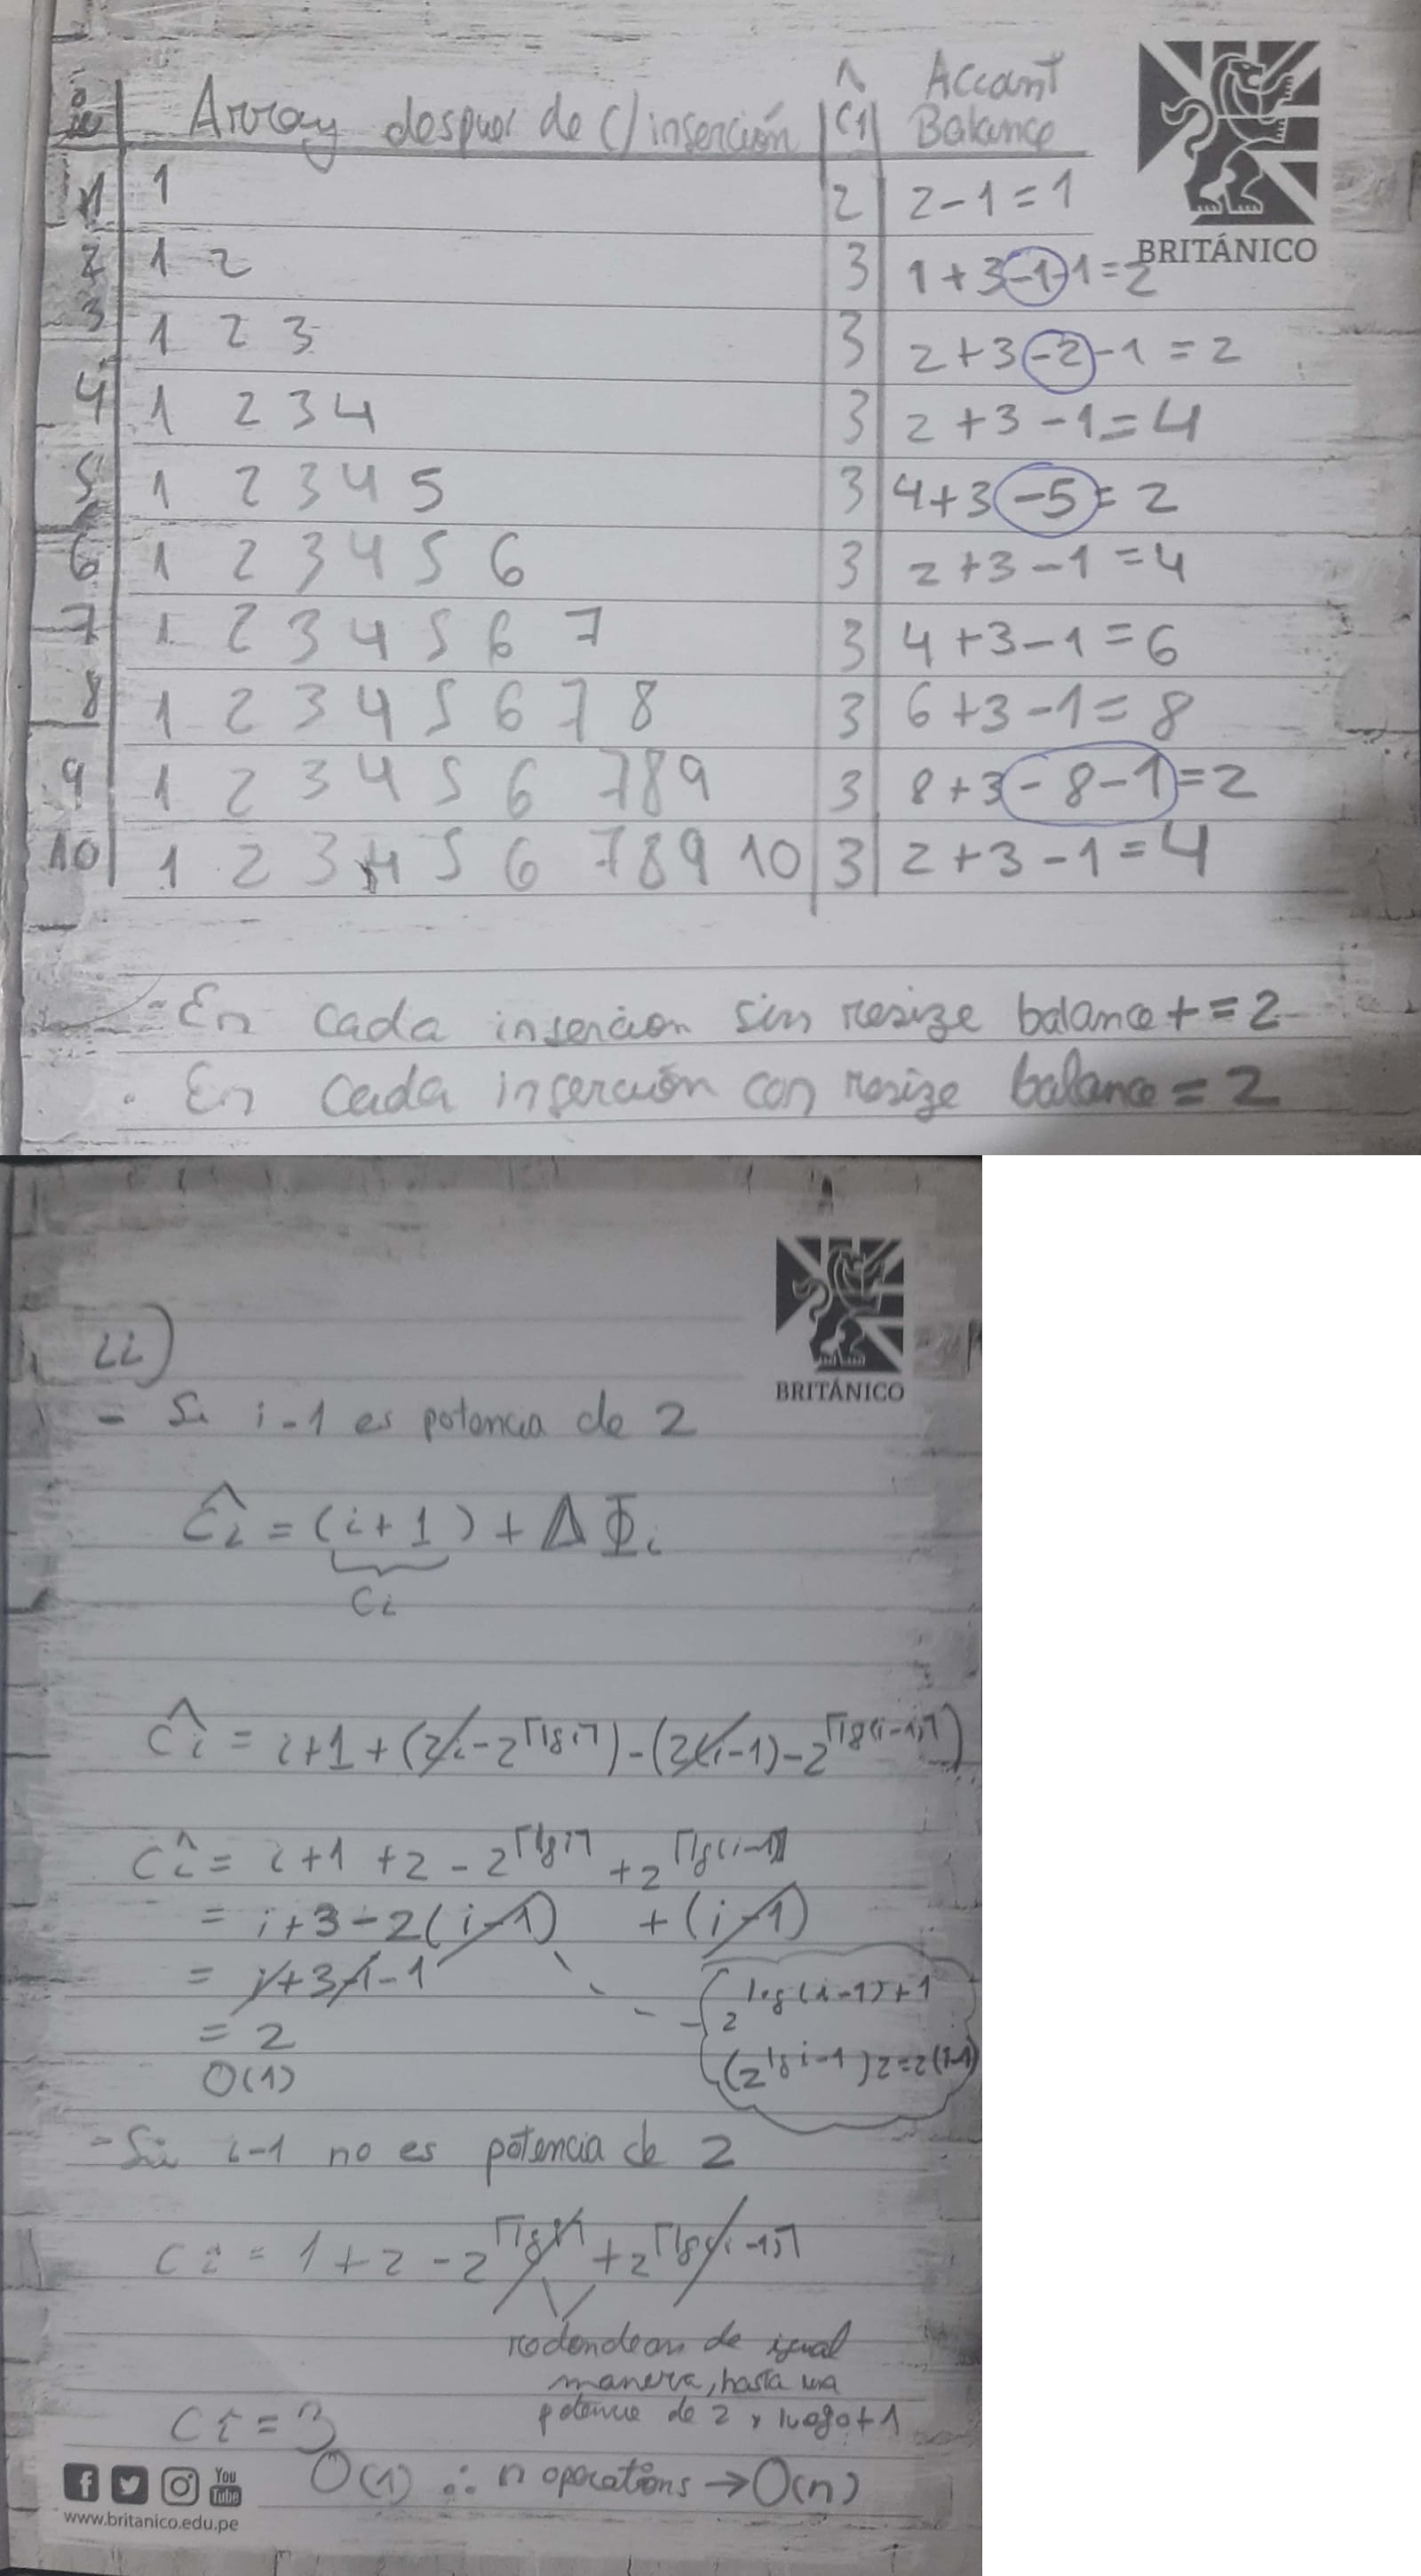
\includegraphics[width=0.7\textwidth]{problem1/problem1}
    \end{figure}

\end{problem}

\begin{problem}{Outcomes a}{5}
    Evaluate the following expressions using Master Method. If the Master Method can't be applied explain the reason.

    \begin{enumerate}[label=(\roman*)]
        \item $T(n) = 20T(n/6) - n^{2}log(n)$
        \item $T(n) = 4T(n/2) + \frac{n}{log(n)}$
        \item $T(n) = 6T(n/3) + n^{2}log(n)$
        \item $T(n) = \sqrt{2}T(n/2) + log(n)$
        \item $T(n) = 2T(n/2) + nlog(n)$
    \end{enumerate}

    \begin{figure}[H]
        \centering
        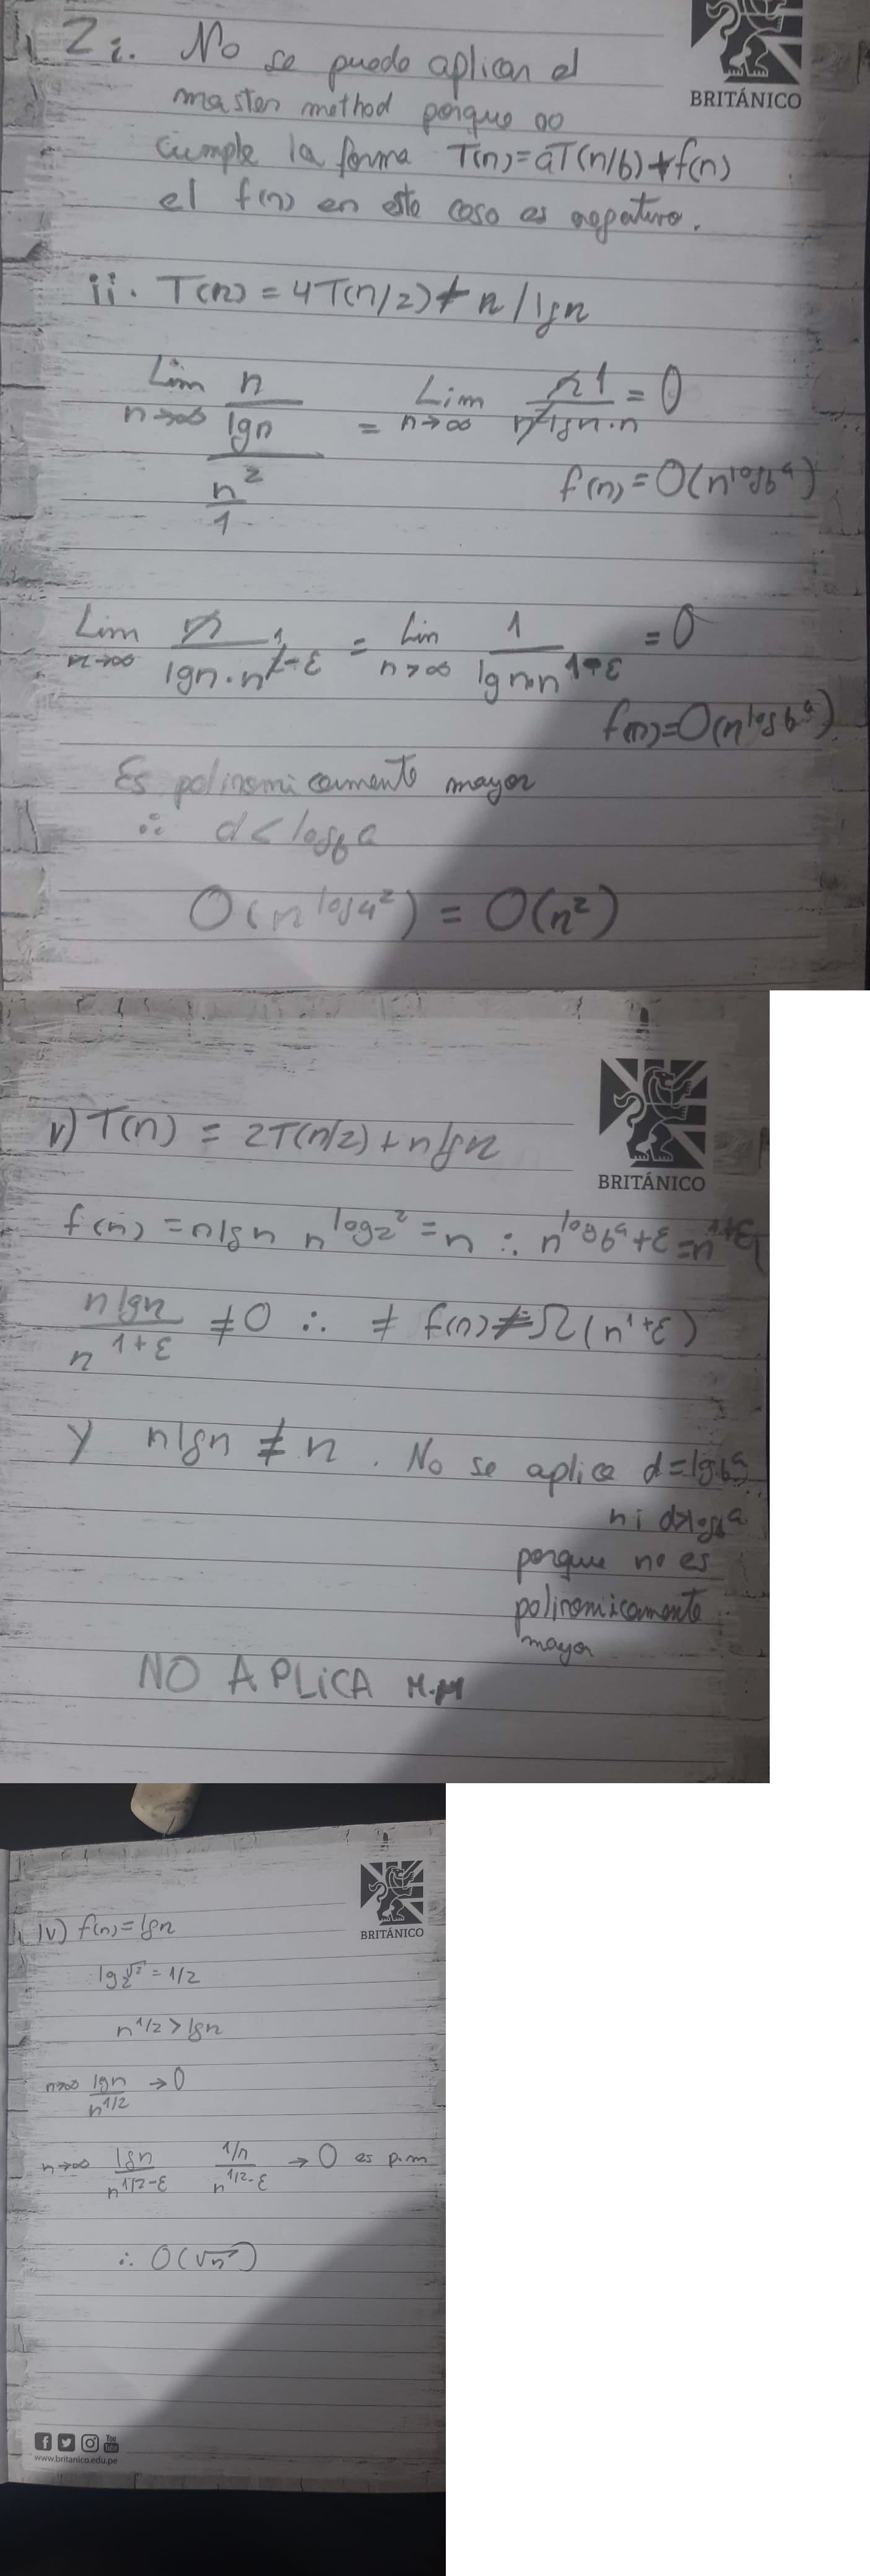
\includegraphics[width=0.7\textwidth]{problem2/problem2}
    \end{figure}
\end{problem}

\begin{problem}{Outcomes a}{4}
    Consider a binary counter algorithm that counts from 0 to n using binary representation. Find an upper bound on the total worst-case running time (1pt), then calculate the amortized cost of each operation using one of the methods presented in class (3pts). Explain your procedure.

    \begin{figure}[H]
        \centering
        
\includegraphics[width=0.7\textwidth]{problem3/problem3}
    \end{figure}
\end{problem}

\begin{problem}{Outcomes a}{2}
    Given $T(n) = 4T(n/3) + n$ prove using substitution method that the solution for this recurrence is $O(n^{log_3 4})$

    \begin{figure}[H]
        \centering
        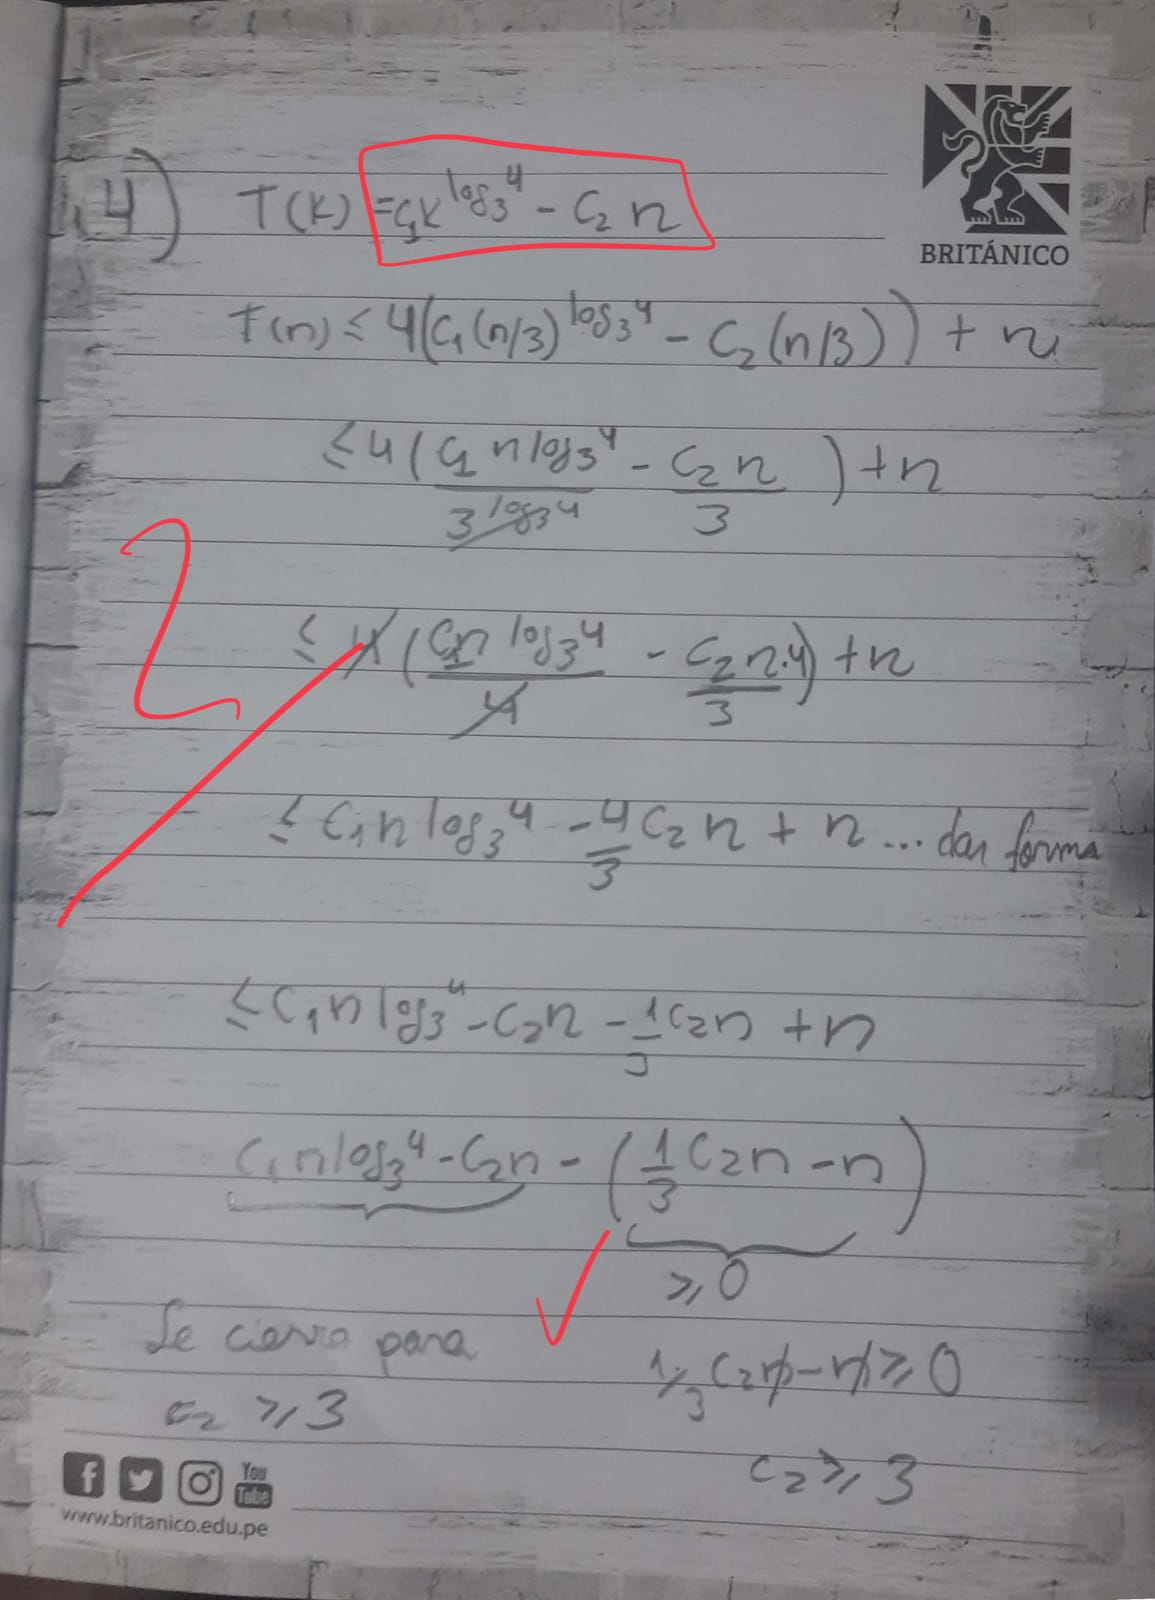
\includegraphics[width=0.7\textwidth]{problem4/problem4}
    \end{figure}
\end{problem}

\begin{problem}{Outcomes a}{4}
    Write a divide-and-conquer c++ algorithm (3pts) that receives and array of $n$ strings and returns the largest prefix of all strings in the array. For example if the array is \{``dog", ``doggie", ``dogs"\} then the largest prefix is ``dog". If there isn't a common prefix between all words return an empty string. After that, write the execution time of your algorithm (1pt)

    \inputminted[fontsize=\small,breaklines]{cpp}{answers/problem5/problem5.cpp}
 \begin{figure}[H]
        \centering
        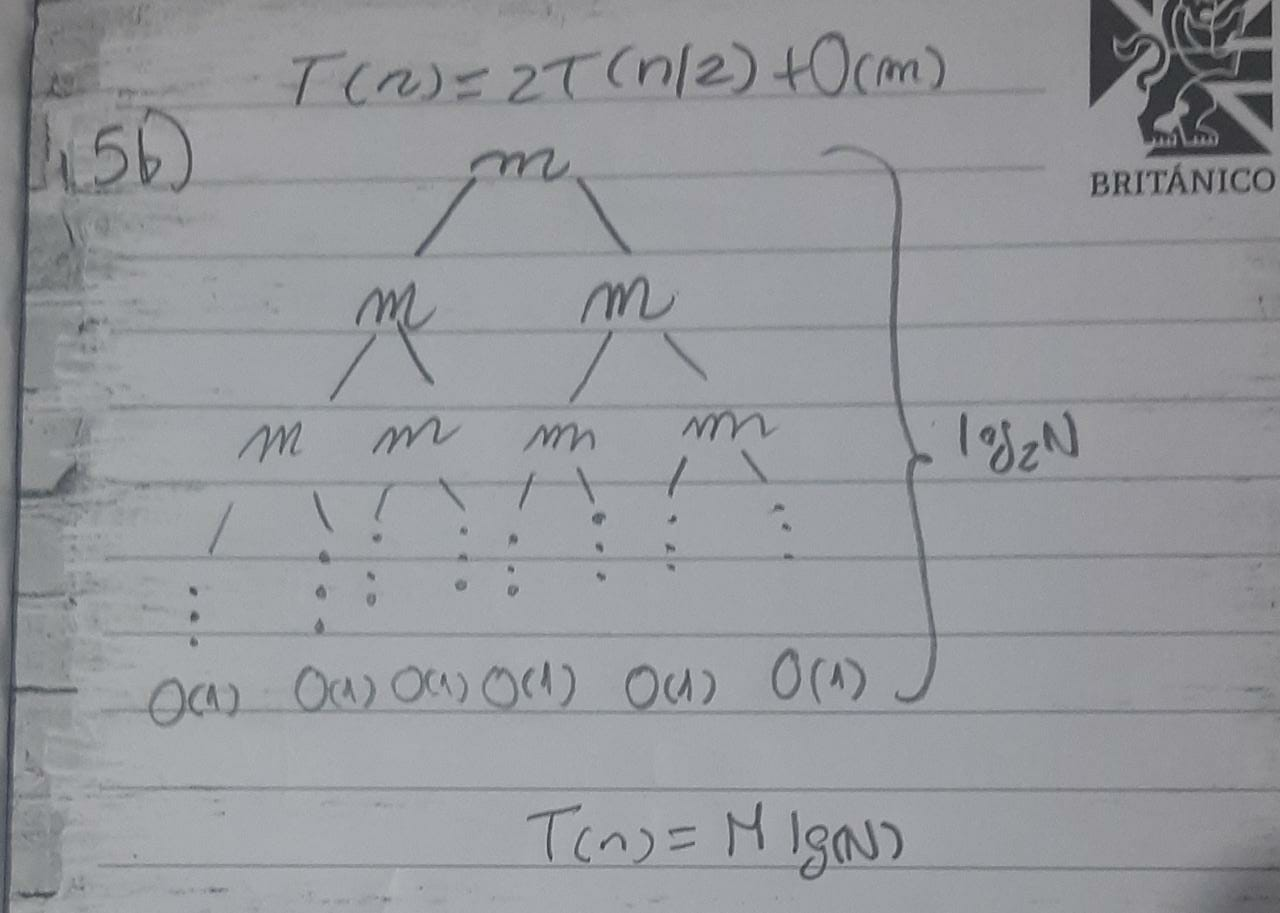
\includegraphics[width=0.7\textwidth]{problem5/problem5}
    \end{figure}

\end{problem}

\end{document}
